% questions.tex —— 2006 年·全国卷Ⅰ·理科 · 题目内容片段（无答案）
% 由 tools/generate_projects.py 依来源总账自 2006/2006_数学真题_全国1理_试题.md 生成，勿手改（改源 MD 后重跑）


\gkpart{数学}

\begin{gktip}
\textbf{来源说明}：本题面依据固定源 PDF 两页 A3 题面逐题转录，原卷印刷页码 312–313。固定源不附答案，答案和解析均由本库独立复算。

\textbf{图形说明}：第 19 题的原卷图形关系重绘为 TikZ/PGFPlots 矢量图。图形标记所指的 PNG 不随仓库保存。
\end{gktip}

\gkpart{一、选择题}

\begin{question}
\gkti{1}设集合 $M=\{x\mid x^2-x<0\}$，$N=\{x\mid |x|<2\}$，则\mbox{（　　）}

（A）$M\cap N=\varnothing$\quad（B）$M\cap N=M$\quad（C）$M\cup N=M$\quad（D）$M\cup N=\mathbb R$

\end{question}
\begin{question}
\gkti{2}已知函数 $y=e^x$ 的图象与函数 $y=f(x)$ 的图象关于直线 $y=x$ 对称，则\mbox{（　　）}

（A）$f(2x)=e^{2x}\ (x\in\mathbb R)$\quad（B）$f(2x)=\ln2\cdot\ln x\ (x>0)$

（C）$f(2x)=2e^x\ (x\in\mathbb R)$\quad（D）$f(2x)=\ln x+\ln2\ (x>0)$

\end{question}
\begin{question}
\gkti{3}双曲线 $mx^2+y^2=1$ 的虚轴长是实轴长的 $2$ 倍，则 $m=$\mbox{（　　）}

（A）$-\dfrac14$\quad（B）$-4$\quad（C）$4$\quad（D）$\dfrac14$

\end{question}
\begin{question}
\gkti{4}如果复数 $(m^2+i)(1+mi)$ 是实数，则实数 $m=$\mbox{（　　）}

（A）$1$\quad（B）$-1$\quad（C）$\sqrt2$\quad（D）$-\sqrt2$

\end{question}
\begin{question}
\gkti{5}函数 $f(x)=\tan\left(x+\dfrac\pi4\right)$ 的单调增区间为\mbox{（　　）}

（A）$\left(k\pi-\dfrac\pi2,k\pi+\dfrac\pi2\right)$，$k\in\mathbb Z$

（B）$(k\pi,(k+1)\pi)$，$k\in\mathbb Z$

（C）$\left(k\pi-\dfrac{3\pi}4,k\pi+\dfrac\pi4\right)$，$k\in\mathbb Z$

（D）$\left(k\pi-\dfrac\pi4,k\pi+\dfrac{3\pi}4\right)$，$k\in\mathbb Z$

\end{question}
\begin{question}
\gkti{6}$\triangle ABC$ 的内角 $A,B,C$ 的对边分别为 $a,b,c$，若 $a,b,c$ 成等比数列，且 $c=2a$，则 $\cos B=$\mbox{（　　）}

（A）$\dfrac14$\quad（B）$\dfrac34$\quad（C）$\dfrac{\sqrt2}4$\quad（D）$\dfrac{\sqrt2}3$

\end{question}
\begin{question}
\gkti{7}已知各顶点都在一个球面上的正四棱柱高为 $4$，体积为 $16$，则这个球的表面积是\mbox{（　　）}

（A）$16\pi$\quad（B）$20\pi$\quad（C）$24\pi$\quad（D）$32\pi$

\end{question}
\begin{question}
\gkti{8}抛物线 $y=-x^2$ 上的点到直线 $4x+3y-8=0$ 距离的最小值是\mbox{（　　）}

（A）$\dfrac43$\quad（B）$\dfrac75$\quad（C）$\dfrac85$\quad（D）$3$

\end{question}
\begin{question}
\gkti{9}设平面向量 $\boldsymbol a_1,\boldsymbol a_2,\boldsymbol a_3$ 的和 $\boldsymbol a_1+\boldsymbol a_2+\boldsymbol a_3=0$。如果向量 $\boldsymbol b_1,\boldsymbol b_2,\boldsymbol b_3$ 满足 $|\boldsymbol b_i|=2|\boldsymbol a_i|$，且 $\boldsymbol a_i$ 顺时针旋转 $30^\circ$ 后与 $\boldsymbol b_i$ 同向，其中 $i=1,2,3$，则\mbox{（　　）}

（A）$-\boldsymbol b_1+\boldsymbol b_2+\boldsymbol b_3=0$\quad（B）$\boldsymbol b_1-\boldsymbol b_2+\boldsymbol b_3=0$

（C）$\boldsymbol b_1+\boldsymbol b_2-\boldsymbol b_3=0$\quad（D）$\boldsymbol b_1+\boldsymbol b_2+\boldsymbol b_3=0$

\end{question}
\begin{question}
\gkti{10}设 $a_n$ 是公差为正数的等差数列，若 $a_1+a_2+a_3=15$，$a_1a_2a_3=80$，则 $a_{11}+a_{12}+a_{13}=$\mbox{（　　）}

（A）$120$\quad（B）$105$\quad（C）$90$\quad（D）$75$

\end{question}
\begin{question}
\gkti{11}用长度分别为 $2,3,4,5,6$（单位：cm）的 $5$ 根细木棒围成一个三角形（允许连接，但不允许折断），能够得到的三角形的最大面积为\mbox{（　　）}

（A）$8\sqrt5\ \mathrm{cm}^2$\quad（B）$6\sqrt{10}\ \mathrm{cm}^2$\quad（C）$3\sqrt{55}\ \mathrm{cm}^2$\quad（D）$20\ \mathrm{cm}^2$

\end{question}
\gkpart{二、填空题}

\begin{question}
\gkti{12}设集合 $I=\{1,2,3,4,5\}$。选择 $I$ 的两个非空子集 $A$ 和 $B$，要使 $B$ 中最小的数大于 $A$ 中最大的数，则不同的选择方法共有\gkblank{}种。（用数字作答）

\end{question}
\begin{question}
\gkti{13}已知正四棱锥的体积为 $12$，底面对角线长为 $2\sqrt6$，则侧面与底面所成的二面角等于\gkblank{}。

\end{question}
\begin{question}
\gkti{14}设 $z=2y-x$，式中变量 $x,y$ 满足下列条件：

\nopagebreak[4]
\[
\begin{cases}
2x-y\geqslant-1,\\
3x+2y\leqslant23,\\
y\geqslant1,
\end{cases}
\]

则 $z$ 的最大值为\gkblank{}。

\end{question}
\begin{question}
\gkti{15}安排 $7$ 位工作人员在 $5$ 月 $1$ 日至 $5$ 月 $7$ 日值班，每人值班一天，其中甲、乙二人都不安排在 $5$ 月 $1$ 日和 $2$ 日，不同的安排方法共有\gkblank{}种。（用数字作答）

\end{question}
\begin{question}
\gkti{16}函数 $f(x)=\cos(\sqrt3x+\varphi)\ (0<\varphi<\pi)$。若 $f(x)+f'(x)$ 是奇函数，则 $\varphi=$\gkblank{}。

\end{question}
\gkpart{三、解答题}

\begin{question}
\gkti{17}$\triangle ABC$ 的三个内角为 $A,B,C$，求当 $A$ 为何值时，$\cos A+2\cos\dfrac{B+C}{2}$ 取得最大值，并求出这个最大值。

\end{question}
\begin{question}
\gkti{18}$A,B$ 是治疗同一种疾病的两种药，用若干试验组进行对比试验。每个试验组由 $4$ 只小白鼠组成，其中 $2$ 只服用 A，另 $2$ 只服用 B，然后观察疗效。若在一个试验组中，服用 A 有效的小白鼠的只数比服用 B 有效的多，就称该试验组为甲类组。设每只小白鼠服用 A 有效的概率为 $\dfrac23$，服用 B 有效的概率为 $\dfrac12$。

（1） 求一个试验组为甲类组的概率；

（2） 观察 $3$ 个试验组，用 $\xi$ 表示这 $3$ 个试验组中甲类组的个数，求 $\xi$ 的分布列和数学期望。

\Needspace{0.4\textheight}
\end{question}
\begin{question}
\gkti{19}如图，$l_1,l_2$ 是互相垂直的异面直线，$MN$ 是它们的公垂线段。点 $A,B$ 在 $l_1$ 上，$C$ 在 $l_2$ 上，$AM=MB=MN$。
\nopagebreak[4]
\begin{center}% 2006 年全国卷Ⅰ理科第 19 题：互相垂直的异面直线
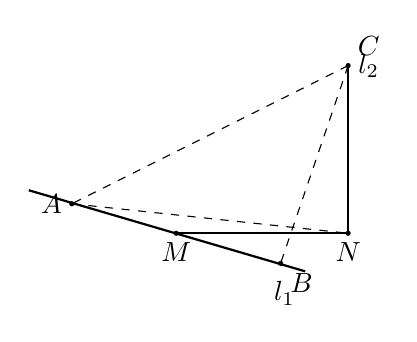
\begin{tikzpicture}[>=stealth,scale=0.78]
  \coordinate (A) at (0.55,1.20);
  \coordinate (M) at (2.25,0.72);
  \coordinate (B) at (3.95,0.23);
  \coordinate (N) at (5.05,0.72);
  \coordinate (C) at (5.05,3.45);
  \draw[thick] (-0.15,1.42)--(4.35,0.10) node[below left] {$l_1$};
  \draw[thick] (N)--(C) node[right] {$l_2$};
  \draw[thick] (M)--(N);
  \draw[dashed] (A)--(N) (C)--(A) (C)--(B);
  \fill (A) circle (1.2pt) node[left] {$A$};
  \fill (M) circle (1.2pt) node[below] {$M$};
  \fill (N) circle (1.2pt) node[below] {$N$};
  \fill (B) circle (1.2pt) node[below right] {$B$};
  \fill (C) circle (1.2pt) node[above right] {$C$};
\end{tikzpicture}
\end{center}
\nopagebreak[4]
（1） 证明：$AC\perp NB$；

（2） 若 $\angle ACB=60^\circ$，求 $NB$ 与平面 $ABC$ 所成角的余弦值。

\end{question}
\begin{question}
\gkti{20}在平面直角坐标系 $xOy$ 中，有一个以 $F_1(0,-\sqrt3)$ 和 $F_2(0,\sqrt3)$ 为焦点、离心率为 $\dfrac{\sqrt3}{2}$ 的椭圆，设椭圆在第一象限的部分为曲线 $C$。动点 $P$ 在 $C$ 上，$C$ 在点 $P$ 处的切线与 $x,y$ 轴的交点分别为 $A,B$，且向量 $\overrightarrow{OM}=\overrightarrow{OA}+\overrightarrow{OB}$。求：

（1） 点 $M$ 的轨迹方程；

（2） $|\overrightarrow{OM}|$ 的最小值。

\end{question}
\begin{question}
\gkti{21}已知函数 $f(x)=\dfrac{1+x}{1-x}e^{-ax}$。

（1） 设 $a>0$，讨论 $y=f(x)$ 的单调性；

（2） 若对任意 $x\in(0,1)$ 恒有 $f(x)>1$，求 $a$ 的取值范围。

\end{question}
\begin{question}
\gkti{22}设数列 $\{a_n\}$ 的前 $n$ 项的和为 $S_n=\dfrac43a_n-\dfrac13\times2^{n+1}+\dfrac23$，$n=1,2,3,\ldots$。

（1） 求首项 $a_1$ 与通项 $a_n$；

（2） 设 $T_n=\dfrac{2^n}{S_n}$，$n=1,2,3,\ldots$，证明：$\displaystyle\sum_{i=1}^nT_i<\dfrac32$。

\end{question}